%%%%  TEIL B: MATHEMATIK LESEN UND SPRECHEN  %%%%
\newpage
\part{Mathematik lesen und sprechen}

In diesem Teil steht, wie man Zeichen, Formeln und Rechenwege auf Englisch (und zum Vergleich auf
Deutsch) vorliest. Links steht der Ausdruck, rechts die englische Lesart und darunter grau die
deutsche. Wo es mehrere übliche Lesarten gibt, sind sie durch Schrägstriche getrennt. Die Beispiele
sind bewusst einfach gehalten, damit sie sich direkt im Unterricht verwenden lassen.

%--------------------------------------------------------------------------------------------------
\section{Zahlen, Zeichen und Schreibweisen}

\subsection*{Ordnungszahlen, Indizes und Aufzählungen}

\begin{lesen}
\lies{1.\quad 2.\quad 3.\quad 21.}{1st, 2nd, 3rd, 21st -- first, second, third, twenty-first}{erstens, zweitens, drittens -- der Erste, der Zweite, \ldots}
\lies{1.\ \ldots, 2.\ \ldots}{firstly \ldots, secondly \ldots}{erstens \ldots, zweitens \ldots}
\lies{$x_1,\ x_2$}{$x$ one, $x$ two \;/\; $x$ sub one, $x$ sub two}{$x$ eins, $x$ zwei \;/\; $x$ Index eins}
\lies{$a_n$}{$a$ sub $n$ \;/\; $a$ $n$}{$a$ Index $n$ \;/\; $a$ $n$}
\lies{$1;\ 2;\ 3;\ \ldots$}{one, two, three, and so on (to infinity)}{eins, zwei, drei und so weiter (unbegrenzt)}
\lies{$1;\ 2;\ \ldots;\ 25$}{one, two, and so on up to twenty-five}{eins, zwei und so weiter bis fünfundzwanzig}
\end{lesen}

\subsection*{Dezimalzahlen, große Zahlen und Brüche}

Im Englischen trennt ein \textbf{Punkt} die Nachkommastellen ab, das Komma gliedert große Zahlen in
Dreiergruppen -- im Deutschen ist es genau umgekehrt. Das führt leicht zu Verwechslungen.

\begin{lesen}
\lies{$3{,}14$ \newline \footnotesize engl. 3.14}{three point one four}{drei Komma eins vier}
\lies{$0{,}3$ \newline \footnotesize engl. 0.3 oder .3}{nought point three \ipa{nO:t} \;/\; zero point three \;/\; point three}{null Komma drei}
\lies{$30\,000$ \newline \footnotesize engl. 30,000}{thirty thousand}{dreißigtausend}
\lies{$2{,}5 \cdot 10^6$ \newline \footnotesize engl. $2.5 \times 10^6$}{two point five times ten to the (power of) six}{zwei Komma fünf mal zehn hoch sechs}
\lies{$\frac12;\ \frac13;\ \frac14$}{a half, a third, a quarter}{ein Halb, ein Drittel, ein Viertel}
\lies{$\frac34;\ \frac58$}{three quarters (AE: three fourths), five eighths}{drei Viertel, fünf Achtel}
\lies{$\frac{1}{100}$}{one hundredth}{ein Hundertstel}
\lies{$\frac{17}{25}$}{seventeen over twenty-five \;/\; seventeen twenty-fifths}{siebzehn Fünfundzwanzigstel}
\end{lesen}

\subsection*{Britisches und amerikanisches Englisch}

Die Lautschrift im Wörterbuch folgt dem britischen Englisch. Im amerikanischen Englisch heißen
einige Dinge anders:

\begin{lesen}
\lies{\textbf{Mathematik}}{maths (BE) \;/\; math (AE)}{}
\lies{$0$}{nought, zero (BE) \;/\; zero (AE)}{}
\lies{$(\ \ )\quad[\ \ ]$}{brackets, square brackets (BE) \;/\; parentheses, brackets (AE)}{}
\lies{Trapez}{trapezium (BE) \;/\; trapezoid (AE)}{}
\lies{$\dfrac34$}{three quarters (BE) \;/\; three fourths (AE)}{}
\lies{Schreibung}{factorise, centre (BE) \;/\; factorize, center (AE)}{}
\end{lesen}

\anmerkung{In englischsprachigen Texten steht zwischen zwei Zahlen meist das Kreuz: $3 \times 5$. Ein
mittiger Punkt kann in älteren britischen Texten als Dezimalpunkt gemeint sein ($3{\cdot}5 = 3{,}5$).
Zwischen Variablen ist der Malpunkt üblich oder wird ganz weggelassen: $a \cdot b = ab$.}

%--------------------------------------------------------------------------------------------------
\section{Relationszeichen}

\begin{lesen}
\lies{$p = q$}{$p$ equals $q$ \;/\; $p$ is equal to $q$}{$p$ (ist) gleich $q$}
\lies{$a \neq b$}{$a$ is not equal to $b$ \;/\; $a$ does not equal $b$}{$a$ (ist) ungleich $b$ \;/\; $a$ nicht gleich $b$}
\lies{$\pi \approx 3{,}14$}{pi is approximately equal to three point one four}{pi (ist) ungefähr gleich drei Komma eins vier}
\lies{$f(x) \equiv 0$}{$f$ of $x$ is identically equal to zero}{$f$ von $x$ ist identisch gleich null}
\lies{$a < b$}{$a$ is less than $b$}{$a$ (ist) kleiner als $b$}
\lies{$a > b$}{$a$ is greater than $b$}{$a$ (ist) größer als $b$}
\lies{$a \le b$}{$a$ is less than or equal to $b$ \;/\; $a$ is not greater than $b$}{$a$ (ist) kleiner oder gleich $b$ \;/\; höchstens gleich $b$}
\lies{$a \ge b$}{$a$ is greater than or equal to $b$ \;/\; $a$ is not less than $b$}{$a$ (ist) größer oder gleich $b$ \;/\; mindestens gleich $b$}
\lies{$a \ll b$}{$a$ is much less than $b$}{$a$ (ist) viel kleiner als $b$}
\lies{$a \gg b$}{$a$ is much greater than $b$}{$a$ (ist) viel größer als $b$}
\lies{$y \sim x$ \newline \footnotesize engl. $y \propto x$}{$y$ is (directly) proportional to $x$}{$y$ ist (direkt) proportional zu $x$}
\lies{$a : b = c : d$}{$a$ is to $b$ as $c$ is to $d$}{$a$ verhält sich zu $b$ wie $c$ zu $d$}
\lies{$2 \le x \le 5$}{$x$ is greater than or equal to two and less than or equal to five \;/\; $x$ lies between two and five inclusive}{$x$ ist mindestens zwei und höchstens fünf \;/\; $x$ liegt zwischen zwei und fünf (einschließlich)}
\end{lesen}

\anmerkung{Das Zeichen $\sim$ bedeutet im Deutschen „proportional“, in der Geometrie aber „ähnlich“
($\triangle ABC \sim \triangle DEF$, \textit{similar}). Im Englischen schreibt man für
„proportional“ meist $\propto$.}

%--------------------------------------------------------------------------------------------------
\section{Grundrechenarten}

Die Namen der Rechengrößen auf einen Blick:
\[
\ub{a}{summand}{Summand} + \ub{b}{summand}{Summand} = \ub{s}{sum}{Summe}
\qquad\qquad
\ub{a}{minuend}{Minuend} - \ub{b}{subtrahend}{Subtrahend} = \ub{d}{difference}{Differenz}
\]
\[
\ub{a}{factor}{Faktor} \cdot \ub{b}{factor}{Faktor} = \ub{p}{product}{Produkt}
\qquad\qquad
\ub{a}{dividend}{Dividend} : \ub{b}{divisor}{Divisor} = \ub{q}{quotient}{Quotient}
\]

\begin{lesen}
\lies{$a_1 + a_2 = s$}{$a$ one plus $a$ two equals $s$}{$a$ eins plus $a$ zwei gleich $s$}
\lies{$L - l = d$}{capital $L$ minus small $l$ equals $d$}{groß $L$ minus klein $l$ gleich $d$}
\lies{$a \cdot b = c$ \newline \footnotesize engl. auch $a \times b$}{$a$ times $b$ equals $c$ \;/\; $a$ multiplied by $b$ equals $c$}{$a$ mal $b$ gleich $c$}
\lies{$ab = c$}{$a$ $b$ equals $c$}{$a$ $b$ gleich $c$}
\lies{$a : b = c$ \newline \footnotesize engl. auch $a \div b$}{$a$ divided by $b$ equals $c$}{$a$ geteilt durch $b$ gleich $c$ \;/\; $a$ durch $b$ gleich $c$}
\lies{$\dfrac{a}{b} = a/b$}{$a$ over $b$}{$a$ durch $b$ \;/\; $a$ $b$-tel}
\end{lesen}

\subsection*{Beispiele}

\begin{lesen}
\lies{$17 + 8 = 25$}{seventeen plus eight equals twenty-five}{siebzehn plus acht gleich fünfundzwanzig}
\lies{$42 - 15 = 27$}{forty-two minus fifteen is twenty-seven}{zweiundvierzig minus fünfzehn ist siebenundzwanzig}
\lies{$6 \cdot 7 = 42$}{six times seven is forty-two \;/\; six sevens are forty-two}{sechs mal sieben ist zweiundvierzig}
\lies{$56 : 8 = 7$}{fifty-six divided by eight is seven}{sechsundfünfzig geteilt durch acht ist sieben}
\lies{$(3 + 4) \cdot 5 = 35$}{the sum of three and four, multiplied by five, equals thirty-five \;/\; open bracket three plus four close bracket times five}{die Summe aus drei und vier, mal fünf, ist fünfunddreißig \;/\; Klammer auf drei plus vier Klammer zu mal fünf}
\end{lesen}

%--------------------------------------------------------------------------------------------------
\section{Rechnen mit Brüchen}

\begin{lesen}
\lies{$\dfrac{12}{18} = \dfrac{2}{3}$}{twelve eighteenths equals two thirds. \newline \textit{Rule:} To reduce a fraction to its lowest terms, divide the numerator and the denominator by their highest common factor (here 6).}{zwölf Achtzehntel gleich zwei Drittel. \newline \textit{Regel:} Man kürzt einen Bruch, indem man Zähler und Nenner durch dieselbe Zahl dividiert (hier 6).}
\lies{$\dfrac{3}{4} = \dfrac{15}{20}$}{three quarters equals fifteen twentieths. \newline \textit{Rule:} To expand a fraction, multiply the numerator and the denominator by the same number (here 5).}{drei Viertel gleich fünfzehn Zwanzigstel. \newline \textit{Regel:} Man erweitert einen Bruch, indem man Zähler und Nenner mit derselben Zahl multipliziert (hier 5).}
\lies{$\dfrac{2}{3} + \dfrac{1}{4} = \dfrac{8}{12} + \dfrac{3}{12} = \dfrac{11}{12}$}{two thirds plus one quarter equals eight twelfths plus three twelfths equals eleven twelfths. \newline \textit{Rule:} To add (or subtract) unlike fractions, change them into like fractions with the lowest common denominator and then add (or subtract) the numerators.}{zwei Drittel plus ein Viertel gleich acht Zwölftel plus drei Zwölftel gleich elf Zwölftel. \newline \textit{Regel:} Ungleichnamige Brüche macht man zuerst gleichnamig (Hauptnenner) und addiert bzw.\ subtrahiert dann die Zähler.}
\lies{$\dfrac{2}{3} \cdot \dfrac{9}{10} = \dfrac{18}{30} = \dfrac{3}{5}$}{two thirds times nine tenths equals eighteen thirtieths equals three fifths. \newline \textit{Rule:} To multiply two fractions, multiply the numerators together and the denominators together.}{zwei Drittel mal neun Zehntel gleich achtzehn Dreißigstel gleich drei Fünftel. \newline \textit{Regel:} Man multipliziert Zähler mit Zähler und Nenner mit Nenner.}
\lies{$\dfrac{3}{4} : \dfrac{9}{8} = \dfrac{3}{4} \cdot \dfrac{8}{9} = \dfrac{2}{3}$}{three quarters divided by nine eighths equals three quarters times eight ninths equals two thirds. \newline \textit{Rule:} To divide by a fraction, multiply by its reciprocal.}{drei Viertel geteilt durch neun Achtel gleich drei Viertel mal acht Neuntel gleich zwei Drittel. \newline \textit{Regel:} Man dividiert durch einen Bruch, indem man mit seinem Kehrwert multipliziert.}
\lies{$\dfrac{11}{4} = 2\tfrac{3}{4} = 2 + \dfrac{3}{4}$}{eleven quarters equals two and three quarters. \newline \textit{Rule:} To convert an improper fraction into a mixed number, split it into the sum of a whole number and a proper fraction.}{elf Viertel gleich zwei drei Viertel. \newline \textit{Regel:} Einen unechten Bruch schreibt man als gemischte Zahl, indem man ihn in eine ganze Zahl und einen echten Bruch zerlegt.}
\end{lesen}

\anmerkung{„Cancel“ heißt wörtlich „streichen“: \textit{Cancel 6 out of the fraction} -- „Kürze den
Bruch durch 6“. Bei gemischten Zahlen sagt man im Englischen immer \textit{and}: $2\tfrac34$ --
\textit{two and three quarters}.}

%--------------------------------------------------------------------------------------------------
\section{Potenzen, Wurzeln und Logarithmen}

Aus der Gleichung $b^n = c$ lassen sich drei Fragen stellen -- je nachdem, welche Größe gesucht ist:

\begin{center}
\begin{tikzpicture}[font=\small]
	\node[font=\huge] (f) at (0.6,0) {$b^{\,n} = c$};
	\coordinate (b) at ($(f.west)+(0.3,-0.15)$);
	\coordinate (n) at ($(f.north west)+(0.62,-0.2)$);
	\coordinate (c) at ($(f.east)+(-0.2,0.05)$);
	% Namen
	\node[align=center, blue!70!black] (nb) at (-2.4,1.3) {base\\[-2pt]\color{black!60}Basis};
	\node[align=center, blue!70!black] (nn) at (0.2,2.2) {exponent\\[-2pt]\color{black!60}Exponent};
	\node[align=center, blue!70!black] (nc) at (3.9,1.3) {power (value of the power)\\[-2pt]\color{black!60}Potenz(wert)};
	\draw[-{Stealth}, blue!70!black, shorten >=4pt] (nb) -- (b);
	\draw[-{Stealth}, blue!70!black, shorten >=4pt] (nn) -- (n);
	\draw[-{Stealth}, blue!70!black, shorten >=4pt] (nc) -- (c);
	% drei Rechenarten
	\node[align=center] (p) at (-5,-2.2) {\textbf{$c$ gesucht:} $c = b^n$\\ raising to a power\\\color{black!60}Potenzieren};
	\node[align=center] (r) at (0.6,-2.6) {\textbf{$b$ gesucht:} $b = \sqrt[n]{c}$\\ extracting a root\\\color{black!60}Radizieren};
	\node[align=center] (l) at (6,-2.2) {\textbf{$n$ gesucht:} $n = \log_b c$\\ taking the logarithm\\\color{black!60}Logarithmieren};
	\draw[red, thick, -{Stealth}] (0.6,-0.5) -- (p.north east);
	\draw[red, thick, -{Stealth}] (0.6,-0.5) -- (r.north);
	\draw[red, thick, -{Stealth}] (0.6,-0.5) -- (l.north west);
\end{tikzpicture}
\end{center}

\subsection*{Potenzen}
\begin{lesen}
\lies{$b^n$}{$b$ to the power of $n$ \;/\; $b$ to the $n$th (power) \;/\; the $n$th power of $b$}{$b$ hoch $n$}
\lies{$5^2 = 25$}{five squared is twenty-five}{fünf Quadrat \;/\; fünf hoch zwei ist fünfundzwanzig}
\lies{$3^3 = 27$}{three cubed is twenty-seven}{drei hoch drei ist siebenundzwanzig}
\lies{$2^5 = 32$}{two to the power of five equals thirty-two \;/\; two to the fifth equals thirty-two}{zwei hoch fünf gleich zweiunddreißig}
\lies{$b^{-n} = \dfrac{1}{b^n}$}{$b$ to the power of minus $n$ equals one over $b$ to the $n$}{$b$ hoch minus $n$ gleich eins durch $b$ hoch $n$}
\lies{$10^{-3} = 0{,}001$}{ten to the minus three equals nought point nought nought one}{zehn hoch minus drei gleich null Komma null null eins}
\end{lesen}

\subsection*{Wurzeln}
\begin{lesen}
\lies{$\sqrt[n]{c} = b$}{the $n$th root of $c$ is (equal to) $b$}{die $n$-te Wurzel aus $c$ ist gleich $b$}
\lies{$\sqrt{49} = 7$}{the square root of forty-nine is seven}{die (Quadrat-)Wurzel aus neunundvierzig ist sieben}
\lies{$\sqrt[3]{8} = 2$}{the cube root of eight is two}{die dritte Wurzel aus acht ist zwei}
\lies{$\sqrt[4]{81} = 3$}{the fourth root of eighty-one is three}{die vierte Wurzel aus einundachtzig ist drei}
\lies{$\sqrt[n]{c^m} = c^{\frac{m}{n}}$}{the $n$th root of $c$ to the power of $m$ equals $c$ to the power of $m$ over $n$}{die $n$-te Wurzel aus $c$ hoch $m$ gleich $c$ hoch $m$ $n$-tel}
\lies{$\sqrt{a^2 + b^2}$}{the square root of $a$ squared plus $b$ squared}{die Wurzel aus $a$ Quadrat plus $b$ Quadrat}
\end{lesen}

\subsection*{Logarithmen}
\begin{lesen}
\lies{$\log_b c = n$}{the logarithm of $c$ to the base $b$ is $n$ \;/\; log to the base $b$ of $c$ equals $n$}{der Logarithmus von $c$ zur Basis $b$ ist $n$}
\lies{$\log_2 32 = 5$}{log to the base two of thirty-two equals five}{Logarithmus von zweiunddreißig zur Basis zwei gleich fünf}
\lies{$\lg 1000 = 3$}{the common logarithm of one thousand is three \;/\; log one thousand equals three}{der Zehnerlogarithmus (dekadische Logarithmus) von tausend ist drei}
\lies{$\ln \mathrm{e} = 1$}{the natural logarithm of $e$ is one \;/\; log $e$ of $e$ equals one}{der natürliche Logarithmus von e ist eins}
\lies{$\log_b(x \cdot y) = \log_b x + \log_b y$}{the log of a product equals the sum of the logs}{der Logarithmus eines Produkts ist gleich der Summe der Logarithmen}
\end{lesen}

\anmerkung{$\ln x$ liest man im Englischen meist \textit{log $x$} oder \textit{ell en $x$}, $\lg x$ ist
im Englischen unüblich -- dort schreibt man $\log_{10} x$ oder nur $\log x$.}

%--------------------------------------------------------------------------------------------------
\section{Zahlbereiche}

\begin{center}
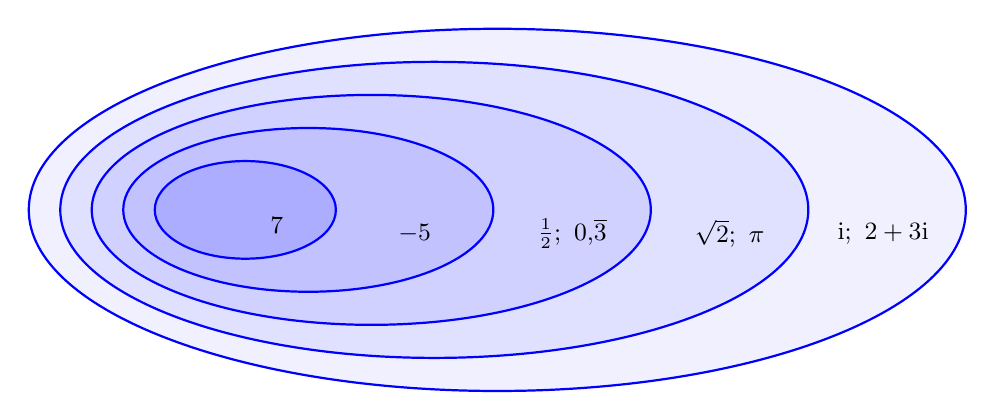
\begin{tikzpicture}[font=\small]
	\foreach \k/\col in {4/blue!6, 3/blue!12, 2/blue!18, 1/blue!24, 0/blue!32} {
		\filldraw[fill=\col, draw=blue, thick] ({0.8*\k},0) ellipse[x radius={1.15+1.2*\k}, y radius={0.62+0.42*\k}];
	}
	\node[font=\large] at (-0.35,0.2) {$\N$};       \node at (0.4,-0.2) {$7$};
	\node[font=\large] at (2.15,0.4) {$\Z$};        \node at (2.15,-0.3) {$-5$};
	\node[font=\large] at (4.15,0.4) {$\Q$};        \node at (4.15,-0.3) {$\frac12;\ 0{,}\overline{3}$};
	\node[font=\large] at (6.15,0.4) {$\R$};        \node at (6.15,-0.3) {$\sqrt2;\ \pi$};
	\node[font=\large] at (8.1,0.4) {$\C$};         \node at (8.1,-0.3) {$\mathrm{i};\ 2 + 3\mathrm{i}$};
\end{tikzpicture}
\end{center}

\begin{lesen}
\lies{$\N = \{0;\ 1;\ 2;\ \ldots\}$}{the set of natural numbers}{die Menge der natürlichen Zahlen}
\lies{$\Z = \{\ldots;\ -1;\ 0;\ 1;\ \ldots\}$}{the set of integers: the union of the positive integers, the negative integers and zero}{die Menge der ganzen Zahlen: positive und negative ganze Zahlen und die Null}
\lies{$\Q = \left\{\dfrac{p}{q} \;\middle|\; p, q \in \Z;\ q \neq 0\right\}$}{the set of all fractions $p$ over $q$, where $p$ and $q$ are integers and $q$ is not zero}{die Menge aller Brüche $p$ durch $q$, wobei $p$ und $q$ ganze Zahlen sind und $q$ ungleich null ist}
\lies{$\R$}{the set of real numbers: all terminating and recurring decimals (rational numbers) and all non-terminating, non-recurring decimals (irrational numbers)}{die Menge der reellen Zahlen: alle abbrechenden und periodischen Dezimalbrüche (rationale Zahlen) und alle nichtabbrechenden, nichtperiodischen Dezimalbrüche (irrationale Zahlen)}
\lies{$\C = \{a + b\,\mathrm{i} \mid a, b \in \R\}$ \newline mit $\mathrm{i}^2 = -1$}{the set of complex numbers: $a$ plus $b$ i, where $a$ and $b$ are real numbers and i is the imaginary unit}{die Menge der komplexen Zahlen: $a$ plus $b$ i, wobei $a$ und $b$ reelle Zahlen sind und i die imaginäre Einheit ist}
\lies{$\N \subset \Z \subset \Q \subset \R \subset \C$}{each number set is a proper subset of the next one}{jeder Zahlbereich ist eine echte Teilmenge des nächsten}
\end{lesen}

\anmerkung{Ob die Null zu den natürlichen Zahlen gehört, wird unterschiedlich gehandhabt. Im Englischen
ist man deshalb oft genauer: \textit{positive integers} ($1;\,2;\,3;\,\ldots$) bzw.\
\textit{non-negative integers} ($0;\,1;\,2;\,\ldots$). Ältere Bücher schreiben noch $N$, $I$, $F$, $R$, $C$ statt
der Doppelstrich-Buchstaben.}

%--------------------------------------------------------------------------------------------------
\section{Mengen}

\begin{lesen}
\lies{$a \in M$}{$a$ is an element of $M$ \;/\; $a$ is in $M$ \;/\; $a$ belongs to $M$}{$a$ ist Element von $M$}
\lies{$a \notin M$}{$a$ is not an element of $M$}{$a$ ist nicht Element von $M$}
\lies{$M = \{2;\ 4;\ 6\}$ \newline \footnotesize engl. $\{2, 4, 6\}$}{$M$ is the set with the elements two, four and six}{$M$ ist die Menge mit den Elementen zwei, vier und sechs}
\lies{$M = \emptyset$}{$M$ is the empty set \;/\; $M$ is a null set}{$M$ ist die leere Menge}
\lies{$A \subseteq B$}{$A$ is a subset of $B$}{$A$ ist (eine) Teilmenge von $B$}
\lies{$A \subset B$}{$A$ is a proper subset of $B$}{$A$ ist (eine) echte Teilmenge von $B$}
\lies{$A \cup B$}{$A$ union $B$ \;/\; the union of $A$ and $B$}{$A$ vereinigt $B$ \;/\; die Vereinigungsmenge von $A$ und $B$}
\lies{$A \cap B$}{$A$ intersection $B$ \;/\; the intersection of $A$ and $B$}{$A$ geschnitten $B$ \;/\; die Schnittmenge von $A$ und $B$}
\lies{$A \setminus B$}{$A$ minus $B$ \;/\; the difference of $A$ and $B$}{$A$ ohne $B$ \;/\; die Differenzmenge von $A$ und $B$}
\lies{$A \times B$}{$A$ cross $B$ \;/\; the Cartesian product of $A$ and $B$}{$A$ kreuz $B$ \;/\; das kartesische Produkt von $A$ und $B$}
\lies{$\{x \in \R \mid x < 4\}$}{the set of all real numbers $x$ such that $x$ is less than four}{die Menge aller reellen Zahlen $x$, für die gilt: $x$ ist kleiner als vier}
\end{lesen}

%--------------------------------------------------------------------------------------------------
\section{Gleichungen und Ungleichungen lösen}

\subsection*{Beispiel: eine lineare Gleichung}

\begin{lesen}
\lies{$\dfrac{2(x - 1)}{3} + \dfrac{1}{2} = \dfrac{5}{2}$}{\textit{Solve the equation.}}{\textit{Löse die Gleichung.}}
\lies{$4(x - 1) + 3 = 15$}{Multiply both sides by the lowest common denominator, six.}{Multipliziere beide Seiten mit dem Hauptnenner sechs.}
\lies{$4x - 4 + 3 = 15$}{Expand the brackets \;/\; remove the parentheses.}{Löse die Klammern auf (multipliziere aus).}
\lies{$4x - 1 = 15$}{Simplify \;/\; collect like terms.}{Fasse zusammen.}
\lies{$4x = 16$}{Add one to both sides.}{Addiere eins auf beiden Seiten.}
\lies{$x = 4$}{Divide both sides by the coefficient of $x$, four.}{Dividiere beide Seiten durch den Koeffizienten von $x$, also durch vier.}
\lies{$L = \{4\}$}{The solution set contains only one element, four. \;/\; The solution is $x$ equals four.}{Die Lösungsmenge enthält nur das Element vier. \;/\; Die Lösung ist $x$ gleich vier.}
\lies{\textit{Probe:} \newline $\frac{2 \cdot 3}{3} + \frac12 = \frac52$ \;\checkmark}{\textit{Check:} Substitute four for $x$: two plus a half equals five halves. \checkmark}{\textit{Probe:} Setze vier für $x$ ein: zwei plus ein Halb gleich fünf Halbe. \checkmark}
\end{lesen}

\subsection*{Beispiel: eine lineare Ungleichung}

\begin{lesen}
\lies{$3 - 2x < 9$}{\textit{Solve the inequality.}}{\textit{Löse die Ungleichung.}}
\lies{$-2x < 6$}{Subtract three from both sides.}{Subtrahiere drei auf beiden Seiten.}
\lies{$x > -3$}{Divide both sides by minus two. \textbf{Remember:} when you multiply or divide by a negative number, the inequality sign is reversed.}{Dividiere beide Seiten durch minus zwei. \textbf{Achtung:} Beim Multiplizieren oder Dividieren mit einer negativen Zahl dreht sich das Relationszeichen um.}
\lies{$L = \{x \in \R \mid x > -3\}$}{The solution set contains all real numbers greater than minus three.}{Die Lösungsmenge enthält alle reellen Zahlen, die größer als minus drei sind.}
\end{lesen}

\begin{center}
\begin{tikzpicture}[scale=0.8, font=\small]
	\draw[achse] (-6.4,0) -- (3.6,0);
	\foreach \x in {-6,...,3} {\draw (\x,0.1) -- (\x,-0.1) node[below] {$\x$};}
	\draw[blue, very thick, -{Stealth}] (-3,0) -- (3.4,0);
	\filldraw[fill=white, draw=blue, very thick] (-3,0) circle (4pt);
	\node[above, blue] at (0.2,0.15) {$x > -3$};
\end{tikzpicture}
\end{center}

\subsection*{Gleichungsarten}

\begin{lesen}
\lies{$3x - 7 = 11$}{a linear equation (an equation of the first degree): three $x$ minus seven equals eleven}{eine lineare Gleichung (Gleichung ersten Grades): drei $x$ minus sieben gleich elf}
\lies{$x^2 - 5x + 6 = 0$}{a quadratic equation (an equation of the second degree): $x$ squared minus five $x$ plus six equals zero}{eine quadratische Gleichung (Gleichung zweiten Grades): $x$ Quadrat minus fünf $x$ plus sechs gleich null}
\lies{$\sqrt{x + 3} = 5$}{a radical equation: the square root of $x$ plus three (the square root of the sum $x$ plus three) equals five}{eine Wurzelgleichung: die Wurzel aus $x$ plus drei (aus der Summe) gleich fünf}
\lies{$2^x = 64$}{an exponential equation: two to the power of $x$ equals sixty-four}{eine Exponentialgleichung: zwei hoch $x$ gleich vierundsechzig}
\lies{$\log_3 x = 4$}{a logarithmic equation: log to the base three of $x$ equals four}{eine logarithmische Gleichung: Logarithmus von $x$ zur Basis drei gleich vier}
\lies{$2 \sin x = 1$}{a trigonometric equation: two sine $x$ equals one}{eine trigonometrische Gleichung: zwei mal Sinus $x$ gleich eins}
\lies{$\dfrac{x - 3}{2x + 1} = \dfrac16$}{$x$ minus three, all over two $x$ plus one, equals one sixth}{$x$ minus drei, alles geteilt durch zwei $x$ plus eins, gleich ein Sechstel}
\end{lesen}

\anmerkung{Bei längeren Brüchen hilft im Englischen \textit{all over}, um zu zeigen, dass der ganze Term
im Zähler steht. Klammern liest man bei Bedarf mit: \textit{open bracket} \ldots\ \textit{close bracket}.}

%--------------------------------------------------------------------------------------------------
\section{Funktionen}

\begin{lesen}
\lies{$y = f(x)$}{$y$ equals $f$ of $x$ \;/\; $y$ is a function of $x$ ($y$ is the value of the function corresponding to $x$)}{$y$ gleich $f$ von $x$ \;/\; $y$ ist der Funktionswert zu $x$}
\lies{$x$}{the independent variable}{die unabhängige Variable}
\lies{$y$}{the dependent variable}{die abhängige Variable}
\lies{$f\colon x \mapsto x^2$}{$f$ maps $x$ to $x$ squared}{$f$ ordnet $x$ das Quadrat von $x$ zu \;/\; $f$: $x$ wird abgebildet auf $x$ Quadrat}
\lies{$f(x) = 2x^2 - 3$}{$f$ of $x$ equals two $x$ squared minus three}{$f$ von $x$ gleich zwei $x$ Quadrat minus drei}
\lies{$f(3) = 15$}{$f$ of three equals fifteen \;/\; the value of $f$ at three is fifteen}{$f$ von drei gleich fünfzehn \;/\; der Funktionswert an der Stelle drei ist fünfzehn}
\lies{$D_f,\ W_f$}{the domain (of definition) and the range of $f$}{der Definitionsbereich und der Wertebereich von $f$}
\end{lesen}

\subsection*{Der Graph einer Funktion}

\begin{center}
\begin{tikzpicture}[font=\small, scale=1.05]
	\draw[achse] (-0.7,0) -- (8.6,0) node[below left] {$x$};
	\draw[achse] (0,-1.1) -- (0,5.4) node[below left] {$y$};
	\begin{scope}
		\clip (-0.7,-1.1) rectangle (8.3,5.2);
		\draw[blue, very thick, domain=-0.35:7.75, samples=80] plot (\x, {0.1*\x*\x*\x - 1.1*\x*\x + 3.2*\x + 0.3});
	\end{scope}
	\coordinate (P) at (6.5,2.0825);
	\draw[red, thick, dashed] (P) -- (6.5,0) (P) -- (0,2.0825);
	\fill[red] (P) circle (2.5pt) node[above left] {$P(x_P \mid y_P)$};
	\node[below] at (6.5,0) {$x_P$}; \node[left] at (0,2.0825) {$y_P$};
	\node[below left] at (0,0) {$O$};
	% Beschriftungen
	\node[align=left, anchor=west] (gr) at (8.0,4.6) {graph of $f$\\\color{black!60}Graph von $f$};
	\draw[-{Stealth}, thin] (gr.west) -- (7.6,4.45);
	\node[align=center] (ab) at (5.1,-1.3) {abscissa \ipa{\ae b\textprimstress sIs@}\\\color{black!60}Abszisse};
	\draw[-{Stealth}, thin] (ab.east) -- (6.35,-0.35);
	\node[align=center] (or) at (-2.0,3.7) {ordinate \ipa{\textprimstress O:dIn@t}\\\color{black!60}Ordinate};
	\draw[-{Stealth}, thin] (or.south) -- (-0.15,2.55);
	\node[align=center] (ur) at (1.6,-1.3) {origin \ipa{\textprimstress 6rIdZIn}\\\color{black!60}Ursprung};
	\draw[-{Stealth}, thin] (ur.north west) -- (-0.1,-0.2);
	\node[align=center] (xa) at (8.6,0.9) {$x$-axis\\\color{black!60}$x$-Achse};
	\node[align=center] (ya) at (1.3,5.3) {$y$-axis\\\color{black!60}$y$-Achse};
\end{tikzpicture}
\end{center}

\begin{lesen}
\lies{$P(x_P \mid y_P)$ \newline \footnotesize engl. $P(x_P, y_P)$}{the point $P$ with the coordinates $x_P$ and $y_P$ in the rectangular (Cartesian) coordinate system}{der Punkt $P$ mit den Koordinaten $x_P$ und $y_P$ im rechtwinkligen (kartesischen) Koordinatensystem}
\lies{$x_P$}{the abscissa (the $x$-coordinate) of $P$}{die Abszisse ($x$-Koordinate) von $P$}
\lies{$y_P$}{the ordinate (the $y$-coordinate) of $P$}{die Ordinate ($y$-Koordinate) von $P$}
\end{lesen}

\subsection*{Einteilung der elementaren Funktionen}

\begin{center}
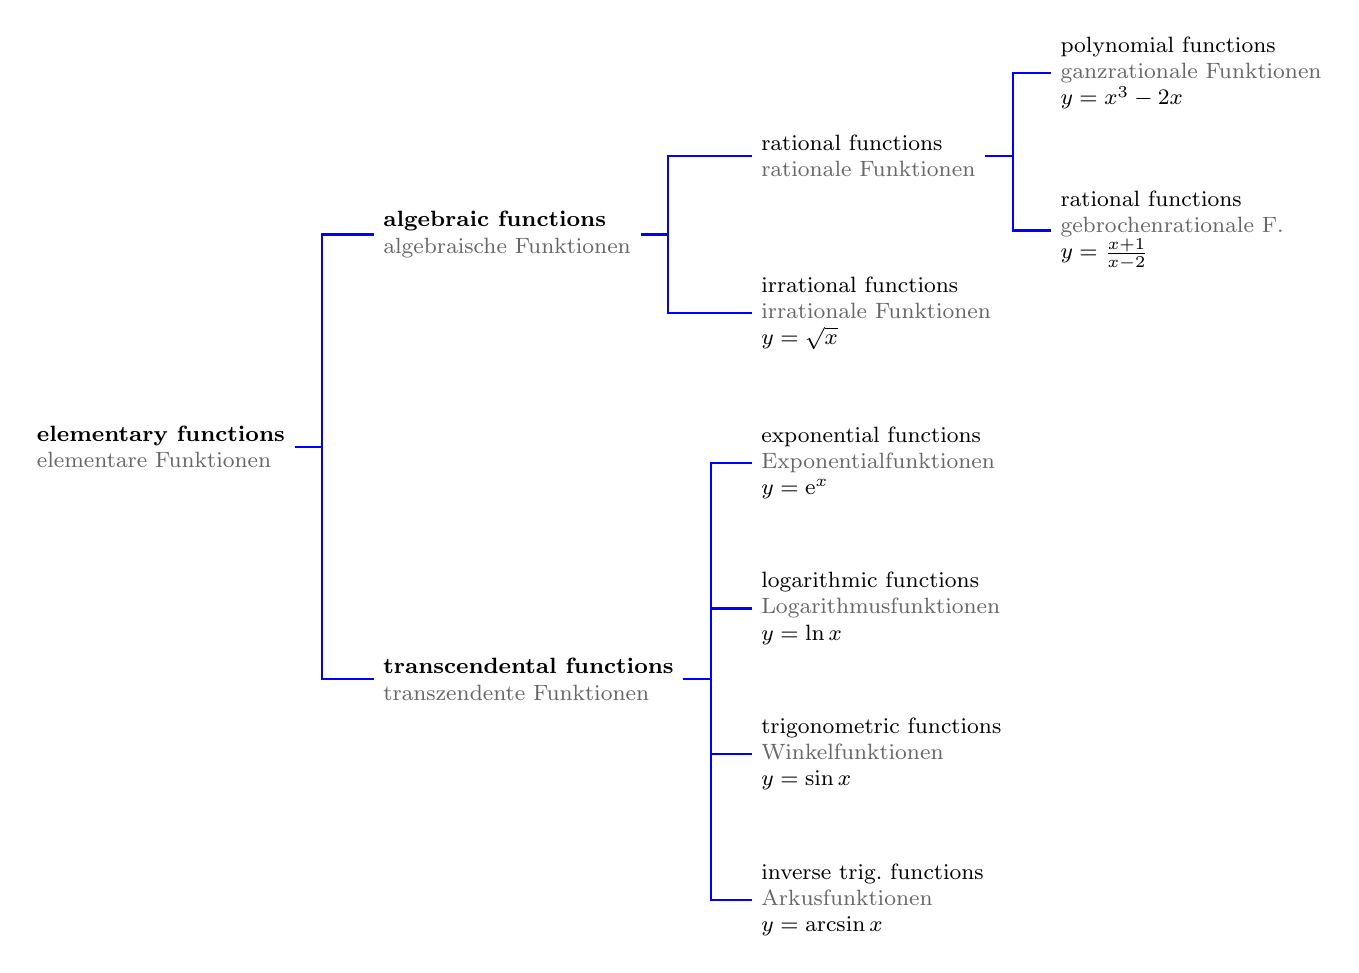
\begin{tikzpicture}[font=\footnotesize, every node/.style={align=left, anchor=west}]
	\node (root) at (0,0)      {\textbf{elementary functions}\\\color{black!60}elementare Funktionen};
	\node (alg) at (4.4,2.7)  {\textbf{algebraic functions}\\\color{black!60}algebraische Funktionen};
	\node (tra) at (4.4,-2.95){\textbf{transcendental functions}\\\color{black!60}transzendente Funktionen};
	\node (rat) at (9.2,3.7)  {rational functions\\\color{black!60}rationale Funktionen};
	\node (irr) at (9.2,1.7)  {irrational functions\\\color{black!60}irrationale Funktionen\\ $y = \sqrt{x}$};
	\node (pol) at (13.0,4.75) {polynomial functions\\\color{black!60}ganzrationale Funktionen\\ $y = x^3 - 2x$};
	\node (fra) at (13.0,2.75) {rational functions\\\color{black!60}gebrochenrationale F.\\ $y = \frac{x + 1}{x - 2}$};
	\node (exp) at (9.2,-0.2) {exponential functions\\\color{black!60}Exponentialfunktionen\\ $y = \mathrm{e}^x$};
	\node (log) at (9.2,-2.05) {logarithmic functions\\\color{black!60}Logarithmusfunktionen\\ $y = \ln x$};
	\node (tri) at (9.2,-3.9) {trigonometric functions\\\color{black!60}Winkelfunktionen\\ $y = \sin x$};
	\node (arc) at (9.2,-5.75) {inverse trig.\ functions\\\color{black!60}Arkusfunktionen\\ $y = \arcsin x$};
	\foreach \a/\b in {root/alg, root/tra, alg/rat, alg/irr, rat/pol, rat/fra, tra/exp, tra/log, tra/tri, tra/arc}
		{\draw[blue, thick] (\a.east) -- ++(0.35,0) |- (\b.west);}
\end{tikzpicture}
\end{center}

\begin{lesen}
\lies{$y = \displaystyle\sum_{k=0}^{4} a_k x^k$}{$y$ equals the sum of $a$ sub $k$ times $x$ to the power of $k$, for $k$ from zero to four}{$y$ gleich Summe über $a$ Index $k$ mal $x$ hoch $k$ für $k$ von null bis vier}
\lies{$y = \dfrac{7 + x}{2 - x^2}$}{$y$ equals the fraction with the numerator seven plus $x$ and the denominator two minus $x$ squared}{$y$ ist gleich dem Bruch mit dem Zähler sieben plus $x$ und dem Nenner zwei minus $x$ Quadrat}
\lies{$y = -\sqrt{r^2 - x^2}$}{$y$ equals the negative square root of $r$ squared minus $x$ squared}{$y$ gleich minus die Wurzel aus $r$ Quadrat minus $x$ Quadrat}
\lies{$y = \mathrm{e}^x$}{$y$ equals $e$ to the (power of) $x$}{$y$ gleich e hoch $x$}
\lies{$y = \ln x$}{$y$ equals log $x$ \;/\; $y$ equals ell en $x$}{$y$ gleich ln $x$ \;/\; $y$ gleich natürlicher Logarithmus von $x$}
\end{lesen}

%--------------------------------------------------------------------------------------------------
\section{Winkelfunktionen}

\begin{center}
\begin{tikzpicture}[scale=2.1, font=\small]
	\draw[achse] (-1.25,0) -- (1.5,0) node[below left] {$x$};
	\draw[achse] (0,-1.2) -- (0,1.35) node[below left] {$y$};
	\draw[blue, thick] (0,0) circle (1);
	\coordinate (P) at (35:1);
	\draw[mass] (0.3,0) arc[start angle=0, end angle=35, radius=0.3]; \node at (17:0.42) {$\alpha$};
	\draw[blue, very thick] (0,0) -- (P);
	\draw[red, very thick] (P) -- (P |- 0,0) node[midway, left, fill=white, inner sep=1pt] {$\sin\alpha$};
	\draw[green!50!black, very thick] (0,0) -- (P |- 0,0) node[midway, below] {$\cos\alpha$};
	\draw[violet, very thick] (1,0) -- (1,{tan(35)}) node[midway, right] {$\tan\alpha$};
	\draw[violet, dashed] (P) -- (1,{tan(35)});
	\fill[blue] (P) circle (1pt) node[above left] {$P$};
	\node[below] at (1,0) {$1$};
	\node[align=left, anchor=west, font=\footnotesize] at (1.55,0.9) {unit circle\\\color{black!60}Einheitskreis};
\end{tikzpicture}
\end{center}

\begin{lesen}
\lies{$\sin x$}{the sine \ipa{saIn} of $x$ \;/\; sine $x$}{Sinus $x$}
\lies{$\cos x$}{the cosine \ipa{"k@UsaIn} of $x$}{Kosinus $x$}
\lies{$\tan x$}{the tangent \ipa{"t\ae ndZ@nt} of $x$ \;/\; tan $x$}{Tangens $x$}
\lies{$\cot x$}{the cotangent \ipa{""k@U"t\ae ndZ@nt} of $x$}{Kotangens $x$}
\lies{$\sec x,\ \csc x$}{the secant \ipa{"si:k@nt} and the cosecant \ipa{""k@U"si:k@nt} of $x$ (in English textbooks also cosec $x$)}{Sekans und Kosekans von $x$ (im deutschen Unterricht kaum verwendet)}
\lies{$\arcsin x$ \newline \footnotesize engl. auch $\sin^{-1} x$}{the inverse sine of $x$ \;/\; arc sine $x$ \;/\; the angle whose sine is $x$}{Arkussinus $x$ \;/\; der Winkel, dessen Sinus $x$ ist}
\lies{$\sin 30\degree = \dfrac12$}{the sine of thirty degrees is one half}{der Sinus von dreißig Grad ist ein Halb}
\lies{$\tan 45\degree = 1$}{the tangent of forty-five degrees equals one}{Tangens fünfundvierzig Grad gleich eins}
\lies{$\sin^2 x + \cos^2 x = 1$}{sine squared $x$ plus cosine squared $x$ equals one}{Sinus Quadrat $x$ plus Kosinus Quadrat $x$ gleich eins}
\lies{$5\sin^2 x - \cos 2x = 0$}{five times the sine squared of $x$, minus the cosine of two $x$, equals zero}{fünf mal Sinus Quadrat $x$ minus Kosinus zwei $x$ ist gleich null}
\end{lesen}

\anmerkung{Vorsicht bei $\sin^{-1} x$: Gemeint ist die Umkehrfunktion $\arcsin x$, nicht der Kehrwert
$\frac{1}{\sin x}$. Auf Taschenrechnern steht dafür ebenfalls oft \textsf{SIN$^{-1}$}.}

%--------------------------------------------------------------------------------------------------
\section{Intervalle und Grenzwerte}

\begin{lesen}
\lies{\intervall{o}{o} \newline $]a;\,b[$ \quad engl. $(a, b)$}{the open interval from $a$ to $b$: $a < x < b$}{das offene Intervall von $a$ bis $b$: $a < x < b$}
\lies{\intervall{g}{g} \newline $[a;\,b]$ \quad engl. $[a, b]$}{the closed interval from $a$ to $b$: $a \le x \le b$}{das abgeschlossene Intervall von $a$ bis $b$: $a \le x \le b$}
\lies{\intervall{o}{g} \newline $]a;\,b]$ \quad engl. $(a, b]$}{the half-open interval from $a$ to $b$, open on the left and closed on the right: $a < x \le b$}{das halboffene Intervall von $a$ bis $b$, links offen und rechts abgeschlossen: $a < x \le b$}
\lies{\intervallR \newline $[a;\,\infty[$ \quad engl. $[a, \infty)$}{the interval from $a$ to infinity: $x \ge a$}{das Intervall von $a$ bis unendlich: $x \ge a$}
\lies{$\R = \ ]{-\infty};\,\infty[$}{the set of real numbers is the open interval from minus infinity to plus infinity}{die Menge der reellen Zahlen ist das offene Intervall von minus unendlich bis plus unendlich}
\end{lesen}

\anmerkung{Im Deutschen sind auch runde Klammern für offene Intervalle verbreitet: $(a;\,b)$. Für
Monotonie-Angaben schreiben wir die Intervalle als Ungleichungskette, z.\,B.\ \textit{fallend:}
$-\infty < x \le 2$.}

\begin{lesen}
\lies{$x \to x_0$}{$x$ tends to $x$ nought \;/\; $x$ approaches $x$ nought}{$x$ gegen $x$ null \;/\; $x$ strebt gegen $x$ null}
\lies{$\limxto{2} x^2 = 4$}{the limit of $x$ squared as $x$ tends to two is four}{der Grenzwert (Limes) von $x$ Quadrat für $x$ gegen zwei ist vier}
\lies{$\limxto{x_1} f(x) = L$}{the limit of $f$ of $x$ as $x$ tends to $x$ one is capital $L$ -- $f(x)$ approaches $L$ as $x$ tends to $x_1$ in any way}{Limes $f$ von $x$ für $x$ gegen $x$ eins ist groß $L$ -- $f(x)$ nähert sich $L$, wenn $x$ beliebig gegen $x_1$ strebt}
\lies{$\limxto{x_0} f(x) \neq f(x_0)$}{the limit of $f$ of $x$ as $x$ tends to $x$ nought is not equal to $f$ of $x$ nought: the function $f$ is discontinuous at $x_0$}{der Grenzwert von $f$ für $x$ gegen $x$ null ist ungleich $f$ von $x$ null: $f$ ist an der Stelle $x_0$ unstetig}
\lies{$\limn \dfrac{1}{n} = 0$}{the limit of one over $n$ as $n$ tends to infinity is zero: $\left(\frac1n\right)$ is a null sequence}{der Grenzwert von eins durch $n$ für $n$ gegen unendlich ist null: $\left(\frac1n\right)$ ist eine Nullfolge}
\lies{$\limn a_n = g$}{the sequence $(a_n)$ converges to $g$ \;/\; the sequence is convergent with the limit $g$}{die Folge $(a_n)$ konvergiert gegen $g$ \;/\; sie ist konvergent mit dem Grenzwert $g$}
\end{lesen}

%--------------------------------------------------------------------------------------------------
\section{Differenzialrechnung}

\begin{center}
\begin{tikzpicture}[scale=1.25, font=\small]
	\draw[achse] (-0.4,0) -- (5,0) node[below left] {$x$};
	\draw[achse] (0,-0.4) -- (0,4.4) node[below left] {$y$};
	\begin{scope}
		\clip (-0.4,-0.4) rectangle (4.8,4.2);
		\draw[blue, very thick, domain=0:4.6, samples=60] plot (\x, {0.2*\x*\x + 0.4});
		% Sekante durch P(1|0,6) und Q(3,5|2,85), Steigung 0,9
		\draw[red, thick, dashed, domain=0:4.8] plot (\x, {0.9*(\x-1) + 0.6});
		% Tangente in P, Steigung 0,4
		\draw[red, very thick, domain=0:4.8] plot (\x, {0.4*(\x-1) + 0.6});
	\end{scope}
	\fill (1,0.6) circle (2pt) node[above left] {$P$};
	\fill (3.5,2.85) circle (2pt) node[above left] {$Q$};
	\draw[black!60] (1,0.6) -- node[below] {$h = \Delta x$} (3.5,0.6) -- node[right] {$\Delta y$} (3.5,2.85);
	\draw[black!40, dotted] (1,0.6) -- (1,0) node[below, black] {$x_0$};
	\draw[black!40, dotted] (3.5,0.6) -- (3.5,0) node[below, black] {$x_0 + h$};
	\node[red, align=left, anchor=west] at (4.85,3.8) {secant \ipa{\textprimstress si:k@nt} -- Sekante};
	\node[red, align=left, anchor=west] at (4.85,2.2) {tangent -- Tangente};
\end{tikzpicture}
\end{center}

\begin{lesen}
\lies{$\dfrac{f(x_0 + h) - f(x_0)}{h}$}{the difference quotient: the slope of the secant through $P$ and $Q$}{der Differenzenquotient: die Steigung der Sekante durch $P$ und $Q$}
\lies{$f'(x_0) = {}$ \newline $\displaystyle\lim_{h \to 0} \frac{f(x_0 + h) - f(x_0)}{h}$}{$f$ prime of $x$ nought is the limit, as $h$ tends to zero, of $f$ of $x$ nought plus $h$ minus $f$ of $x$ nought, all over $h$. Geometrically it is the slope of the tangent at $P$.}{$f$ Strich von $x$ null ist der Grenzwert für $h$ gegen null von $f$ von $x$ null plus $h$ minus $f$ von $x$ null, alles durch $h$. Geometrisch ist das die Steigung der Tangente in $P$.}
\lies{$f'(x),\ f''(x),\ f^{(n)}(x)$}{the first, second, $n$th derivative of $f$ of $x$: $f$ prime of $x$ (or: $f$ dash of $x$), $f$ double prime of $x$, $f$ $n$ prime of $x$}{die erste, zweite, $n$-te Ableitung von $f$: $f$ Strich von $x$, $f$ zwei Strich von $x$, $f$ $n$ Strich von $x$}
\lies{$\dfrac{\mathrm{d}y}{\mathrm{d}x}$}{d $y$ by d $x$ \;/\; d $y$ d $x$ -- the differential quotient of $y$}{d $y$ nach d $x$ -- der Differenzialquotient von $y$}
\lies{$\dfrac{\mathrm{d}^2 y}{\mathrm{d}x^2}$}{d two $y$ by d $x$ squared}{d zwei $y$ nach d $x$ Quadrat}
\lies{$\dfrac{\mathrm{d}^n y}{\mathrm{d}x^n}$}{d $n$ $y$ by d $x$ to the $n$th}{d $n$ $y$ nach d $x$ hoch $n$}
\lies{$\dfrac{\partial z}{\partial x}$}{partial d $z$ by d $x$ \;/\; the partial derivative of $z$ with respect to $x$}{d $z$ partiell nach d $x$}
\lies{$\dot{s} = \dfrac{\mathrm{d}s}{\mathrm{d}t}$}{$s$ dot equals d $s$ by d $t$ (derivative with respect to time)}{$s$ Punkt gleich d $s$ nach d $t$ (Ableitung nach der Zeit)}
\end{lesen}

\subsection*{Beispiele}

\begin{lesen}
\lies{$(x^3)' = 3x^2$}{the derivative of $x$ cubed is three $x$ squared}{die Ableitung von $x$ hoch drei ist drei $x$ Quadrat}
\lies{$(\sin x)' = \cos x$}{the (first) derivative of the sine of $x$ equals the cosine of $x$}{die (erste) Ableitung von Sinus $x$ ist Kosinus $x$}
\lies{$f(x) = x^2 - 4x$ \newline $f'(x) = 2x - 4$}{Differentiate $f$: $f$ prime of $x$ equals two $x$ minus four.}{Leite $f$ ab: $f$ Strich von $x$ gleich zwei $x$ minus vier.}
\lies{$2x - 4 = 0 \ \Rightarrow\ x_E = 2$}{Set the first derivative equal to zero and solve for $x$.}{Setze die erste Ableitung gleich null und löse nach $x$ auf.}
\lies{$f''(2) = 2 > 0$}{The second derivative at two is positive, so the graph has a minimum (a turning point) there: $T(2 \mid -4)$.}{Die zweite Ableitung an der Stelle zwei ist positiv, also hat der Graph dort einen Tiefpunkt: $T(2 \mid -4)$.}
\end{lesen}

%--------------------------------------------------------------------------------------------------
\section{Integralrechnung}

\begin{center}
\begin{tikzpicture}[scale=1.15, font=\small]
	% Untersumme (grau) und Obersumme (rot gestrichelt) für f(x) = 0,15x^2 + 0,6 auf [1; 5], n = 8
	\foreach \i in {0,...,7} {
		\pgfmathsetmacro{\xl}{1+0.5*\i} \pgfmathsetmacro{\xr}{1.5+0.5*\i}
		\pgfmathsetmacro{\yl}{0.15*\xl*\xl+0.6} \pgfmathsetmacro{\yr}{0.15*\xr*\xr+0.6}
		\filldraw[fill=gray!35, draw=gray] (\xl,0) rectangle (\xr,\yl);
		\draw[red, dashed] (\xl,\yl) -- (\xl,\yr) -- (\xr,\yr) -- (\xr,\yl);
	}
	\draw[achse] (-0.4,0) -- (6.2,0) node[below left] {$x$};
	\draw[achse] (0,-0.4) -- (0,5) node[below left] {$y$};
	\draw[blue, very thick, domain=0:5.6, samples=60] plot (\x, {0.15*\x*\x + 0.6}) node[right] {$f$};
	\draw[black!60] (1,0) -- (1,0.75); \draw[black!60] (5,0) -- (5,4.35);
	\node[below] at (1,0) {$a$}; \node[below] at (5,0) {$b$};
	\draw[|<->|, black!70] (3,-0.5) -- node[below] {$\Delta x$} (3.5,-0.5);
	\node[align=left, anchor=west] at (6.4,1.2) {\textcolor{gray}{\rule{8pt}{8pt}} lower sum -- Untersumme\\[2pt] \textcolor{red}{\rule[2pt]{8pt}{0.8pt}} upper sum -- Obersumme};
\end{tikzpicture}
\end{center}

\begin{lesen}
\lies{$\displaystyle\int f(x)\dx = F(x) + C$, \newline wenn $F'(x) = f(x)$}{the integral of $f$ of $x$ d $x$ equals capital $F$ of $x$ plus capital $C$, if capital $F$ prime of $x$ is equal to $f$ of $x$}{Integral $f$ von $x$ d $x$ ist gleich groß $F$ von $x$ plus groß $C$, wenn groß $F$ Strich von $x$ gleich $f$ von $x$ ist}
\lies{$\displaystyle\int f(x)\dx$}{the indefinite integral of $f$; $F$ is an antiderivative of $f$, $C$ is the constant of integration}{das unbestimmte Integral von $f$; $F$ ist eine Stammfunktion von $f$, $C$ die Integrationskonstante}
\lies{$\displaystyle\int_a^b f(x)\dx$}{the integral from $a$ to $b$ of $f$ of $x$ d $x$ -- a definite integral with the lower limit $a$ and the upper limit $b$}{Integral von $a$ bis $b$ über $f$ von $x$ d $x$ -- ein bestimmtes Integral mit der unteren Grenze $a$ und der oberen Grenze $b$}
\lies{$\big[F(x)\big]_a^b = F(b) - F(a)$}{capital $F$ of $x$ between the limits $a$ and $b$ \;/\; $F$ of $x$ evaluated from $a$ to $b$ equals $F$ of $b$ minus $F$ of $a$}{groß $F$ von $x$ in den Grenzen von $a$ bis $b$ ist gleich $F$ von $b$ minus $F$ von $a$}
\lies{$\displaystyle\lim_{\Delta x \to 0} \sum_{k} f(x_k)\,\Delta x$}{the limit, for delta $x$ tending to zero, of the sum of $f$ of $x$ sub $k$ times delta $x$}{der Grenzwert für Delta $x$ gegen null der Summe über $f$ von $x$ Index $k$ mal Delta $x$}
\lies{$\displaystyle\int_a^b f(x)\dx = A$}{for $f(x) \ge 0$: the area bounded by the graph of $f$, the $x$-axis and the lines $x = a$ and $x = b$}{für $f(x) \ge 0$: der Inhalt der Fläche zwischen dem Graphen von $f$, der $x$-Achse und den Geraden $x = a$ und $x = b$}
\end{lesen}

\subsection*{Beispiele}

\begin{lesen}
\lies{$\displaystyle\int \cos x \dx = \sin x + C$}{the integral of cosine $x$ d $x$ equals sine $x$ plus $C$}{Integral Kosinus $x$ d $x$ gleich Sinus $x$ plus $C$}
\lies{$\displaystyle\int_0^2 x^2 \dx = \left[\tfrac13 x^3\right]_0^2 = \tfrac83$}{the integral from nought to two of $x$ squared d $x$ equals one third $x$ cubed between nought and two, which is eight thirds}{Integral von null bis zwei über $x$ Quadrat d $x$ gleich ein Drittel $x$ hoch drei in den Grenzen von null bis zwei, also acht Drittel}
\lies{$\displaystyle\int_1^{\mathrm{e}} \frac{1}{x} \dx = \big[\ln x\big]_1^{\mathrm{e}} = 1$}{the integral from one to $e$ of one over $x$ d $x$ equals log $x$ from one to $e$, which is one}{Integral von eins bis e über eins durch $x$ d $x$ gleich ln $x$ in den Grenzen von eins bis e, also eins}
\end{lesen}

\anmerkung{Wichtige Anwendungen der Integralrechnung in der Geometrie -- \textit{important applications of
integral calculus in geometry}: Flächeninhalte (\textit{areas}), Volumina (\textit{volumes}
\ipa{\textprimstress v6lju:mz}) und Bogenlängen (\textit{arc lengths} \ipa{A:k}).}
